\chapter{STM32WB5MM-DK razvojni sustav}

Razvojni sustav temelji se na STM32WB5MMG modulu tvrtke \textit{STMicroelectronics}, koji je dio linije STM32WBx5 razvojnih sustava. Kao i svi mikrokontroleri iz te skupine, modul sadrži 32-bitni Arm Cortex-M4, aplikacijski procesor koji radi na frekvenciji do 64 MHz, te Cortex-M0+, mrežni procesor s frekvencijom rada do 32 MHz. Modul sadrži 1 MB \textit{Flash} memorije i 256 KB SRAM-a. Budući da je modul RF primopredajnik, podržava protokole Bluetooth, Zigbee, Thread i konkurentne bežične standarde. Sustav također ima 0.96-inčni 128x64 zaslon, RGB LED lampice te senzore za temperaturu, dodir, I2C, \textit{Time-of-Flight} senzor i žiroskop. Od ostale periferije najznačajniji je digitalni MEMS mikrofon. STM32 modul je višeprotokolni, bežični uređaj niske potrošnje energije (engl. \textit{ultra-low-power}) primarno namijenjen razvoju aplikacija koje koriste audio, USB ili \textit{Bluetooth Low Energy} (BLE) protokol. 

\begin{figure}[ht]
	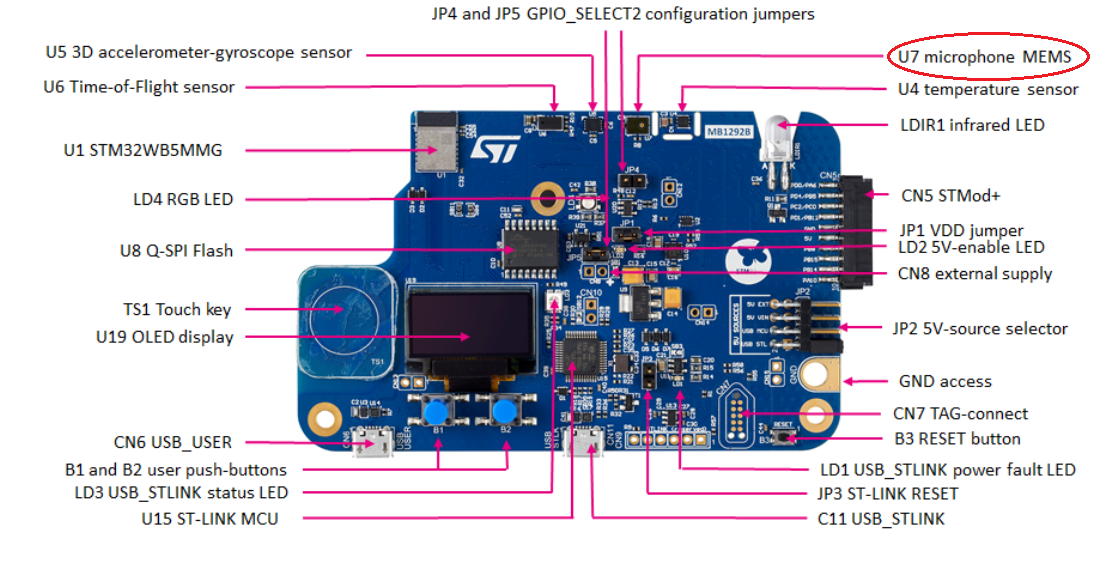
\includegraphics[width=\linewidth]{imgs/discovery_kit}
	\caption{Konfiguracija STM32WB5MM-DK razvojnog sustava}
	\label{fig:discovery-kit}
\end{figure}

\section{BLE protokol}

Bluetooth protokol korišten je za povezivanje razvojnog sustava s matičnim računalom i za prijenos audio signala s mikrokontrolera. BLE je vrsta bežične komunikacije namijenjena komunikaciji kratkog dometa s niskom potrošnjom energije. Razvijen je kako bi se postigao standard vrlo male snage koji radi s baterijom veličine kovanice (engl. \textit{coin-cell batteries}) nekoliko godina.
Klasična Bluetooth tehnologija razvijena je kao bežični standard, što je omogućilo razvoj bežičnih i prenosivih uređaja, no ne podržava dug život baterije zbog brze i nepredvidive komunikacije te složenih postupaka povezivanja. BLE uređaji troše samo dio energije koju troše standardni Bluetooth proizvodi te omogućavaju malenim uređajima s malim baterijama bežično povezivanje s uređajima koji koriste klasični Bluetooth.

BLE radi u istom opsegu od 2,4 GHz kao i standardni Bluetooth, no koristi različite kanale od standardnog Bluetootha. Koristi 40 kanala od 2 MHz za prijenos podataka korištenjem modulacije Gaussova pomaka frekvencije (metoda koja se koristi za glatkije prijelaze između podatkovnih impulsa), zbog čega skokovi frekvencije proizvode manje smetnji u usporedbi sa standardnom Bluetooth komunikacijom.

Arhitektura BLE tehnologije naziva se još i BLE stog zbog slojevite strukture. Stog se sastoji od dvije glavne komponente:
\begin{itemize}
	\item Upravljač (engl. \textit{Controller})
	\item Domaćin (engl. \textit{Host})
\end{itemize}

Upravljač se sastoji od fizičkog sloja i sloja veze. Host uključuje protokol kontrole i prilagodbe logičke veze (L2CAP), upravitelja sigurnosti (SM), protokol atributa (ATT), generički profil atributa (GATT) i generički profil pristupa (GAP). Sučelje između komponenti naziva se sučelje host kontrolera (HCI).


\begin{figure}[ht]
		\centering
		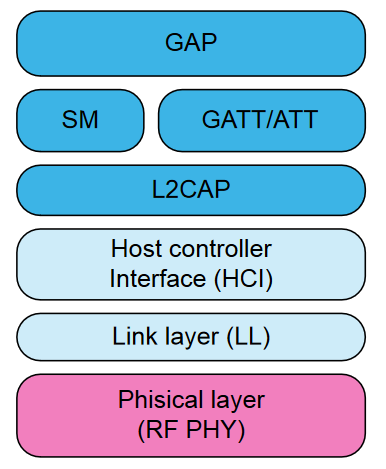
\includegraphics[scale=0.5]{imgs/ble_stack_arch}
		\caption{BLE arhitektura stoga}
		\label{fig:ble-stack-arch}
\end{figure}

\subsection{Upravljač}
\subsubsection{Fizički sloj}
Fizički sloj je radio brzine od 1 Mbps koji prenosi informacije GFSK (\textit{ Gaussian Frequency Shift Keying}) frekvencijskom modulacijom. Radi u 2,4 GHz ISM pojasu bez licence na 2400-2483,5 MHz. 
BLE sustav koristi 40 RF kanala (0-39), s razmakom od 2 MHz. Postoje dvije vrste kanala:
\begin{enumerate}
	\item Kanali za oglašavanje koji koriste tri fiksna RF kanala (37, 38 i 39) za
	\begin{enumerate}
		\item Pakete kanala za oglašavanje
		\item Pakete korištene za otkrivanje ili povezivanje
		\item Pakete korištene za odašiljanje ili skeniranje
	\end{enumerate}
	\item Podatkovni fizički kanal, koristi ostalih 37 RF kanala za dvosmjernu komunikaciju između povezanih uređaja.
\end{enumerate}

BLE je tehnologija adaptivnog skakanja frekvencije (AFH) koja može koristiti samo podskup svih dostupnih frekvencija kako bi se izbjegle sve frekvencije koje koriste druge neprilagodljive tehnologije. To omogućuje prelazak s lošeg kanala na poznati dobar kanal korištenjem specifičnog algoritma za skakanje frekvencije, koji određuje sljedeći dobar kanal za korištenje.

\subsubsection{Sloj veze}
Sloj veze određuje kako dva uređaja mogu koristiti radio za međusoban prijenos informacija. Također definira automat s pet stanja:
\begin{itemize}
	\item Stanje pripravnosti (engl. \textit{Standby}): uređaj ne šalje niti prima pakete
	\item Oglašavanje: uređaj šalje oglase putem kanala za oglašavanje
	\item Skeniranje: uređaj traži uređaje oglašivača
	\item Pokretanje (iniciranje): uređaj pokreće vezu s uređajem oglašivača
	\item Veza: uređaj inicijatora u glavnoj je ulozi (engl. \textit{master}) - komunicira s uređajem u podređenoj (engl. \textit{slave}) ulozi i definira vrijeme prijenosa
	\item Uređaj oglašivača je u ulozi podređenog - komunicira s jednim uređajem u glavnoj ulozi 
\end{itemize}

\begin{figure}[ht]
	\centering
	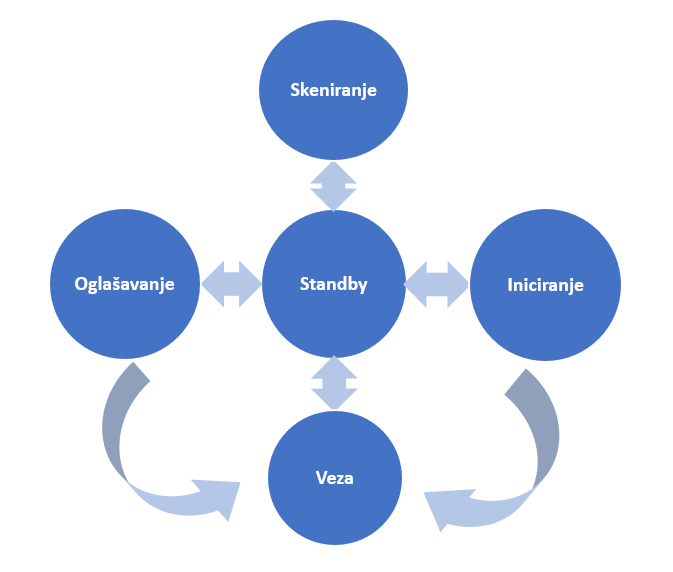
\includegraphics[]{imgs/ll_state_machine}
	\caption{Automat sloja veze}
	\label{fig:ll-state-machine}
\end{figure}

\subsubsection{HCI}
Sloj sučelja glavnog kontrolera (HCI) pruža sredstvo komunikacije između hosta i upravljača  putem softverskog API-ja ili hardverskog sučelja kao što su: SPI, UART ili USB. Dolazi iz standardnih Bluetooth specifikacija, s novim dodatnim naredbama za funkcije specifične uz nisku potrošnju energije.

\subsection{Domaćin}

\subsubsection{L2CAP}
Protokol logičke veze i sloja prilagodbe (L2CAP) podržava multipleksiranje protokola više razine, operacije fragmentacije paketa i ponovnog sastavljanja, te prijenos informacija o kvaliteti usluga.

\subsubsection{ATT}
Protokol atributa (ATT) omogućuje uređaju da prikazuje podatke, koji se nazivaju atributima, drugom uređaju. Uređaj koji prikazuje atribute naziva se poslužiteljem, a uređaj koji ih koristi naziva se klijentom. 
ATT definira skup metoda za otkrivanje, čitanje i pisanje atributa na drugi uređaj. Implementira \textit{peer-to-peer} protokol između poslužitelja i klijenta tipičnom zahtjev-odgovor strukturom. Poslužitelj i klijent imaju sljedeće uloge: 
\begin{itemize}
	\item Poslužitelj
	\begin{itemize}
		\item Sadrži sve atribute (baza atributa)
		\item Prima zahtjeve, šalje odgovore, izvršava naredbe
		\item Obavijesti o promjeni vrijednosti atributa
	\end{itemize}
	\item Klijent
	\begin{itemize}
		\item Komunicira s poslužiteljem
		\item Šalje zahtjeve, čeka na odgovor
		\item Može čitati i mijenjati podatke uz dopuštenje poslužitelja
	\end{itemize}
\end{itemize}

\subsubsection{SM}
BLE sloj veze podržava enkripciju i autentifikaciju korištenjem načina brojača s CBC-MAC algoritmom (kod za provjeru autentičnosti lančanih poruka) i 128-bitnu AES blok šifru (AES-CCM). Kada se enkripcija i autentifikacija koriste u vezi, 4-bajtna provjera integriteta poruke (MIC) dodaje se korisnom učitavanju podatkovnog kanala PDU. Enkripcija se primjenjuje i na polja od PDU i MIC. Kada dva uređaja žele šifrirati komunikacije tijekom veze, upravitelj sigurnosti (SM) koristi postupak uparivanja. Ovaj postupak omogućuje provjeru autentičnosti dvaju uređaja razmjenom informacija o njihovu identitetu kako bi se stvorili sigurnosni ključevi koji se mogu koristiti kao osnova za pouzdani odnos ili (jednu) sigurnu vezu. 

\subsubsection{GATT}
Generički atributni profil (GATT) definira okvir za korištenje ATT protokola, a koristi se za usluge, otkrivanje deskriptora, čitanje, pisanje i obavijesti. U GATT kontekstu, kada su dva uređaja povezana, postoje dvije uloge uređaja:
\begin{itemize}
	\item GATT klijent: uređaj pristupa podacima na udaljenom GATT poslužitelju putem čitanja, pisanja, obavještavanja 
	\item  GATT poslužitelj: uređaj pohranjuje podatke lokalno i pruža metode pristupa podacima udaljenom GATT klijentu
\end{itemize}

Uređaj istovremeno može biti i GATT poslužitelj i GATT klijent.

\subsubsection{GAP}
Bluetooth sustav definira osnovni profil koji implementiraju svi Bluetooth uređaji koji se naziva generički profil pristupa (GAP), koji definira osnovne zahtjeve Bluetooth uređaja. Postoje četiri uloge GAP profila:
\begin{itemize}
	\item Emiter: šalje oglase
	\item Promatrač: prima oglase
	\item Periferija: uvijek u načinu oglašavanja i u \textit{slave} ulozi 
	\item Centar: nikada ne šalje oglase, uvijek u \textit{master} ulozi
\end{itemize}

U kontekstu GAP-a definirana su dva temeljna koncepta:
\begin{itemize}
	\item GAP načini rada (engl. \textit{modes}): konfigurira uređaj da djeluje na određeni način duži vremenski period. Postoje četiri tipa GAP načina rada: emitiranje, otkrivanje, povezivanje i vezanje
	\item GAP procedure: konfigurira uređaj da izvrši jednu radnju u ograničenom vremenskom periodu. Postoje četiri tipa GAP postupaka: promatrač, otkrivanje, povezivanje, postupci povezivanja
\end{itemize}

Istovremeno se mogu koristiti različiti načini otkrivanja i povezivanja.

\section{MEMS mikrofon}